\documentclass[sigconf]{acmart}

\settopmatter{printacmref=false}
\renewcommand\footnotetextcopyrightpermission[1]{}
\pagestyle{plain}

\usepackage{graphicx}
\usepackage[table]{xcolor}
\usepackage{array}
\usepackage{url}
\usepackage{booktabs}
\usepackage{mathtools}
\usepackage{amsthm}
\usepackage{balance}
\usepackage{multirow}

\newtheorem{definition}{Definition}
\newtheorem{problem}{Problem}

\newcommand{\method}{EmbedOpt}
\newcommand{\ndcg}{nDCG@10}
\newcommand{\bpv}{\mathrm{bytes/vec}}
\newcommand{\HV}{\mathrm{HV}}

\acmConference[EDBT 2027]{28th International Conference on Extending Database Technology}{Experiments, Analysis \& Benchmarks}{TBD}


\title{[EA\&B] Benchmarking Embedding Compression for Efficient Neural Retrieval}

\author{Jorge Martinez-Gil}
\affiliation{%
  \institution{Software Competence Center Hagenberg GmbH}
  \city{Hagenberg}
  \postcode{4232}
  \country{Austria}}
\email{jorge.martinez-gil@scch.at}

\begin{abstract}
Vector databases store one dense embedding per object, and that embedding column is usually the largest materialized structure they manage. Choosing how to store it---raw float, halved precision, scalar quantization, product quantization, or a composition of these---trades quality, memory, and latency in ways that depend on the backbone, workload, and budget. We treat this as a physical-design problem and build \method{}, a benchmark that enumerates a search space of post-hoc compression operators (float32, float16, scalar int8, binary, PQ, OPQ, truncation, and compositions), measures each under a common protocol, and emits a Pareto-filtered catalog with paired bootstrap confidence intervals, randomization $p$-values, and codebook-seed variance. On nine BEIR pairs covering E5-base, BGE-base, and MXBAI-large over SciFact, NFCorpus, and ArguAna, scalar int8 saves $4\times$ storage with no statistically significant \ndcg{} loss at $\alpha{=}0.05$ on any pair; float16 saves $2\times$ at the same null. At looser quality budgets, PQ, OPQ, binary, and truncate--PQ reach $48\times$--$128\times$ reductions, and the best layout depends on backbone and dataset. A worked 50M-vector E5-base example shows the same catalog returning three different deployment choices under three different RAM and quality constraints, without rerunning any sweep.
\end{abstract}

\begin{CCSXML}
<ccs2012>
 <concept>
  <concept_id>10002951.10003317.10003347</concept_id>
  <concept_desc>Information systems~Retrieval models and ranking</concept_desc>
  <concept_significance>500</concept_significance>
 </concept>
 <concept>
  <concept_id>10002951.10003260.10003277</concept_id>
  <concept_desc>Information systems~Data layout</concept_desc>
  <concept_significance>500</concept_significance>
 </concept>
 <concept>
  <concept_id>10002951.10003317.10003331</concept_id>
  <concept_desc>Information systems~Search engine architectures and scalability</concept_desc>
  <concept_significance>300</concept_significance>
 </concept>
</ccs2012>
\end{CCSXML}

\ccsdesc[500]{Information systems~Retrieval models and ranking}
\ccsdesc[500]{Information systems~Data layout}
\ccsdesc[300]{Information systems~Search engine architectures and scalability}

\keywords{vector databases, embedding compression, physical design, product quantization, Pareto optimization, retrieval systems, reproducibility}

\begin{document}
\maketitle
\pagestyle{plain}

\section{Introduction}
\label{sec:intro}

Dense text embeddings power semantic search, retrieval-augmented generation, deduplication, clustering, recommendation, and feature stores~\cite{karpukhin2020dpr,lewis2020rag,reimers2019sbert}. A vector database stores one embedding per object and scores incoming queries against the collection at interactive latency. The embedding column is typically the largest materialized structure such a system manages~\cite{pan2024vectordb,zilliztech2021milvus}: a 1\,M-document corpus at 4096 bytes per float32 vector occupies roughly 4\,GB before any index overhead, and the same arithmetic scales to hundreds of gigabytes once corpora reach tens or hundreds of millions of vectors.

How that column is stored---raw float, halved precision, a reduced-dimensional projection, a quantized code, or a chain of these---is therefore a deployment-critical choice. Current practice often resolves it once, at engineering time: a team picks a target codec, checks whether quality loss is ``acceptable,'' and ships. This hides two facts. First, many compressed representations are mutually incomparable along quality, bytes, and latency, so single-metric evaluation discards the shape of the trade-off. Second, quality changes from compression are often within the sampling noise of the test workload; without per-query significance testing, a near-lossless codec is indistinguishable from an underspecified one.

We treat post-hoc embedding compression as a physical-design problem for vector collections, in the spirit of relational physical-design advisors~\cite{chaudhuri1997self,agrawal2004autoadmin}. Given a frozen embedder, a workload, and relevance labels, the goal is not to pick one universally best compressor but to recover the Pareto frontier of vector layouts over retrieval quality, storage, and latency, with statistical uncertainty against the uncompressed baseline. Operators select a deployment point from this frontier under their own constraints.

We instantiate this view in \method{}, a reproducible framework that:

\begin{itemize}
  \item formalizes post-hoc embedding compression as layout selection over $(Q, B, L)$ and produces a statistically annotated catalog of non-dominated layouts (Sections~\ref{sec:problem}--\ref{sec:method});
  \item evaluates a unified search space of float32, float16, truncation, scalar int8, binary, PQ, OPQ, and truncate--PQ / truncate--binary compositions under one protocol, with paired bootstrap CIs, paired randomization $p$-values, and across-seed codebook variance (Sections~\ref{sec:method}--\ref{sec:system});
  \item benchmarks the resulting layouts against six ANN backends spanning exact, IVF, IVF-PQ, HNSW, and OPQ designs (Section~\ref{sec:ann-backends});
  \item reports a 3\,$\times$\,3 BEIR matrix (E5-base, BGE-base, MXBAI-large on SciFact, NFCorpus, ArguAna), extended to FiQA and TREC-COVID on E5-base, with per-pair Pareto sets and hypervolume scores (Sections~\ref{sec:setup}--\ref{sec:results}).
\end{itemize}

The headline empirical finding is bounded but clean. Across all nine pairs, scalar int8 yields a $4\times$ storage reduction with no statistically significant \ndcg{} loss at $\alpha{=}0.05$; float16 yields $2\times$ at the same null. At stricter quality budgets the catalog selects int8 or float16 everywhere, while at looser budgets it switches to PQ, OPQ, binary, or composed layouts whose identity depends on the backbone and workload. The systems message is that those switches are budget-dependent and should be cataloged, not memorized as a single codec rule.

\paragraph{Scope.} We benchmark compression operators and FAISS-backed ANN indexes. We do not benchmark database-native engines (pgvector, Milvus, Qdrant, OpenSearch) directly; we map our results to documented production analogs in those systems via their published storage-mode definitions. The contribution is a benchmark of the compression layer that those systems share, not a competitive comparison among DBMS products.

\section{Background and Related Work}
\label{sec:related}

\subsection{Vector databases and retrieval workloads.}
Vector database management systems organize, index, and serve dense embedding collections~\cite{pan2024vectordb,zilliztech2021milvus,douze2024faiss}, exposing top-$k$ similarity search via exact dense scoring or an approximate nearest-neighbor (ANN) index such as HNSW~\cite{malkov2020hnsw} or IVF~\cite{baranchuk2018revisiting}. Retrieval quality is evaluated on BEIR~\cite{thakur2021beir} and MTEB~\cite{muennighoff2023mteb}; system-side benchmarks such as ANN-Benchmarks~\cite{aumuller2017annbenchmarks} and FAISS~\cite{douze2024faiss,johnson2019billion} target recall/latency at fixed embeddings. We sit between these traditions: backbones and BEIR datasets are fixed; the vector \emph{representation} and the index backend are swept.

\subsection{Dense embedding backbones.}
Sentence-transformer backbones such as E5~\cite{wang2022e5}, BGE / C-Pack~\cite{xiao2023cpack}, and MXBAI-large~\cite{mxbai2024embed} provide strong general-purpose retrieval quality without fine-tuning. We treat them as frozen embedding functions; \method{} does not retrain, finetune, distill, or replace any backbone.

\subsection{Vector compression.}
Three families dominate. \emph{Dimensionality reduction}, including Matryoshka representation learning~\cite{kusupati2022matryoshka}, exposes a contiguous prefix as a lower-dimensional vector. \emph{Scalar quantization} discretizes each dimension into a small number of bits; the production endpoints are IEEE-754 binary16 (pgvector \texttt{halfvec}, Milvus \texttt{FLOAT16}, Qdrant \texttt{Float16}) and 8-bit affine quantization (FAISS \texttt{IndexScalarQuantizer}, Milvus \texttt{SQ8}). \emph{Vector quantization}---product quantization (PQ)~\cite{jegou2011product}, optimized PQ (OPQ)~\cite{ge2014opq}, anisotropic VQ~\cite{guo2020faisspq}---splits a vector into subspaces and stores codebook IDs. Binary embeddings push this to one bit per dimension. Production systems often combine these (e.g., IVF--PQ in FAISS~\cite{douze2024faiss}, link-and-code~\cite{douze2019linkndcode}). We use these operators as physical-design primitives and benchmark their composition under a common workload-aware objective vector.

\subsection{Multi-objective optimization.}
Pareto dominance and the dominated hypervolume indicator~\cite{zitzler1999multiobjective} are standard tools for comparing multi-objective solutions; NSGA-II~\cite{deb2002fast} is a canonical search procedure. The search space evaluated here is enumerable, so exact Pareto filtering and hypervolume suffice; NSGA-style search would be relevant for larger composed spaces.

\subsection{Physical design and IR evaluation.}
Choosing materialized representations under a workload is the classical physical-design problem in databases~\cite{chaudhuri1997self,agrawal2004autoadmin,idreos2018dataalchemist}. We carry that framing to vector retrieval. On the IR side, paired bootstrap and paired randomization are the standard tests for comparing per-query \ndcg{} deltas~\cite{smucker2007comparison,efron1986bootstrap}, and we report both.

\section{Problem Formulation}
\label{sec:problem}

Let $E$ be a frozen text embedder mapping an object $x$ to a vector $E(x) \in \mathbb{R}^{d}$. Let $D = \{d_i\}_{i=1}^{n}$ be a corpus, $Q = \{q_j\}_{j=1}^{m}$ a query workload, and $R$ relevance judgments. A compressor (or \emph{vector layout}) $c \in \mathcal{C}$ specifies a fitting procedure on corpus vectors, an encoding map for corpus and query vectors, and a scoring function over the resulting compressed representations.

For each layout $c$, \method{} measures
\begin{align}
  Q(c) &= \ndcg(c; E, D, Q, R),\\
  B(c) &= \bpv(c; E, D),\\
  L(c) &= \mathrm{median\_query\_latency\_ms}(c; E, D, Q).
\end{align}

\begin{definition}[Dominance]
Layout $c_a$ dominates $c_b$ if it is no worse on every objective and strictly better on at least one. Under the canonical minimization vector $\mathbf{f}(c) = [-Q(c),\, B(c),\, L(c)]$, $c_a$ dominates $c_b$ iff $\mathbf{f}(c_a) \le \mathbf{f}(c_b)$ component-wise with at least one strict inequality.
\end{definition}

The Pareto frontier $\mathcal{P}(\mathcal{C})$ is the set of non-dominated layouts. The dominated hypervolume~\cite{zitzler1999multiobjective} relative to a fixed reference point $\mathbf{r}$ in the same objective space is
\begin{equation}
  \HV(\mathcal{P}; \mathbf{r}) = \mathrm{vol}\!\left( \bigcup_{c \in \mathcal{P}} \prod_{k=1}^{3} [f_k(c), r_k] \right).
\end{equation}

A constrained selection problem then reads:
\begin{problem}[Constrained layout selection]
\label{prob:constrained}
Given budgets $B_{\max}, L_{\max}$ and a quality-loss tolerance $\epsilon$, return $\arg\max_{c \in \mathcal{C}} Q(c)$ subject to $B(c) \le B_{\max}$, $L(c) \le L_{\max}$, and $Q(\mathrm{identity}) - Q(c) \le \epsilon$.
\end{problem}

\paragraph{The layout-advisor catalog.}
The artifact \method{} maintains for a (backbone, workload) pair is a statistically annotated table with schema
\[
\text{(\texttt{spec}, } Q, B, L, \Delta Q_{95\%CI}, p, \sigma_{\text{seed}}, \texttt{is\_pareto}).
\]
$\sigma_{\text{seed}}$ is populated for codebook-trained operators (PQ, OPQ) by the seed-variance sweep of Section~\ref{sec:seed-variance} and is zero for the deterministic operators (identity, float16, scalar int8, binary). The catalog supports four operations: filter by constraint ($B \le B_{\max}$, $L \le L_{\max}$, $Q_{\mathrm{identity}} - Q \le \epsilon$); filter by dominance (\texttt{is\_pareto}); filter by significance ($p \ge \alpha$ \emph{and} $|\Delta Q| > k \cdot \sigma_{\text{seed}}$); and argmax/argmin under constraint. A vector-DB advisor consumes this artifact much as a relational advisor consumes a catalog of candidate physical structures. If the workload or budget changes, the catalog is re-scanned without re-running the backbone or re-training any codec. Section~\ref{sec:advisor-example} walks one such session end-to-end.

\section{Compression Search Space}
\label{sec:method}

Each compression method is a candidate physical layout for the same embedding column. The search space spans conservative layouts that preserve quality, aggressive layouts that minimize storage, and composed layouts that chain dimensional truncation with quantization. All candidates share a uniform interface so they can be evaluated, compared, and recorded in one catalog.

\subsection{Operator interface}
Every operator implements four primitives: \texttt{fit}, \texttt{transform}, \texttt{score}, and \texttt{bytes\_per\_vector}. This contract lets \method{} treat any layout, including composed pipelines, as a single specification string that can be registered, evaluated, persisted, and replayed.

\subsection{Base operators}
\begin{itemize}
  \item \textbf{Identity (float32)}: raw float32 vectors scored with cosine/inner product. Reference for all paired tests.
  \item \textbf{Float16}: IEEE-754 binary16 at 2\,bytes/dim. Scoring upcasts to float32 once per query batch, so the $2\times$ storage saving is decoupled from the scoring path.
  \item \textbf{Truncate}$(k)$: keep the first $k$ dimensions, re-normalize, score in $\mathbb{R}^{k}$. Mirrors deployment use of Matryoshka-style truncation~\cite{kusupati2022matryoshka} on backbones not trained for it.
  \item \textbf{Scalar int8}: per-dimension affine quantization to 8 bits with explicit dequantization at scoring time.
  \item \textbf{Binary}: sign-bit thresholding with Hamming-corrected inner products on packed bits.
  \item \textbf{Product Quantization (PQ)}$(M,b)$: split into $M$ subspaces; learn $2^b$ centroids per subspace with $k$-means; store one code per subspace~\cite{jegou2011product}. Scoring uses asymmetric distance with precomputed query-to-centroid tables. We evaluate $b \in \{4, 6, 8\}$.
  \item \textbf{Optimized PQ (OPQ)}$(M,b)$: a learned orthogonal rotation fit jointly with the PQ codebooks via alternating SVD~\cite{ge2014opq}. At the same byte budget OPQ typically matches or beats PQ. We expose $b \in \{4, 8\}$ over the same $M$ grid; reported bytes equal the packed code size $\lceil M \cdot b / 8 \rceil$.
\end{itemize}

\subsection{Composed operators}
\begin{itemize}
  \item \textbf{Truncate-then-PQ}: \texttt{composed(truncate$(k)$ + PQ$(M,b)$)}. Cheaper codebook training and byte budgets unreachable by PQ alone on high-dim backbones.
  \item \textbf{Truncate-then-binary}: \texttt{composed(truncate$(k)$ + binary)}. Aggressive knob for storage-dominated regimes.
\end{itemize}

For each backbone--dataset pair we evaluate $73$ specifications: identity, float16, 5 truncation cuts, scalar int8, binary, $5\times 3 = 15$ PQ configurations, $5\times 2 = 10$ OPQ configurations, and 39 composed configurations (truncate--PQ and truncate--binary over $k \in \{64,128,256\}$; cells with $M$ exceeding the truncated dimension are skipped). The exact grid is persisted in each run manifest.

\subsection{Objectives, Pareto filtering, statistics}
\textbf{Quality} is per-query \ndcg{}~\cite{jarvelin2002cumulated} aggregated over the workload. For every non-identity layout \method{} reports a paired bootstrap 95\% CI over per-query $\Delta\ndcg = Q(c) - Q(\mathrm{identity})$ with $5000$ resamples and a paired randomization $p$-value with $5000$ resamples~\cite{smucker2007comparison}, both sharing query IDs across the two layouts. For PQ and OPQ we add the across-seed standard deviation $\sigma_{\text{seed}}$ over five training seeds (Section~\ref{sec:seed-variance}).

\textbf{Storage} is the materialized bytes per vector as written by the encoder, including per-codebook overhead amortized over the corpus and packed-code arithmetic at $n_{\text{bits}}<8$ (so PQ$(8, 4)$ reports $4$ bytes/vec).

\textbf{Latency} is the median single-query wall-clock scoring time over the workload (p95 also recorded). It is the cost of the layout under our common scoring path, not the cost of a production-tuned kernel. This separates two questions: representation design (how much quality, storage, and scoring work a layout induces) and ANN-engine design (how a backend realizes that layout). Section~\ref{sec:ann-backends} probes the second axis with six FAISS-family backends.

After evaluation, layouts are filtered to the Pareto-optimal set under $(-Q, B, L)$ and the hypervolume is computed relative to a fixed reference point.

\section{System and Implementation}
\label{sec:system}

\method{} is a Python package (\texttt{embedopt}) with three integration points relevant to data-systems readers. It materializes embeddings for every (backbone, dataset) pair, runs the full sweep, writes per-pair CSV and manifest artifacts, and emits a global \texttt{summary.json}. A CPU-only fallback (\texttt{SCORE\_DEVICE=cpu}) is exercised in CI. BEIR loaders consume standard public splits; the codebook-training seed list is $\{0,1,2,3,4\}$; bootstrap and significance resamples are $5{,}000$ each; profile repeats are $20$.

\paragraph{Embedding cache and spec-level checkpointing.}
Backbone forward passes are the dominant cost. Computed embeddings are persisted by (backbone, dataset) so subsequent sweeps reuse them. Each evaluated specification writes its row to the candidate CSV before the next spec runs, so a sweep can resume after interruption.

\paragraph{Manifest-backed reproducibility.}
Every run writes a JSON manifest containing the configuration, dataset spec, corpus and query counts, list of evaluated specifications, resample counts, the registered Pareto specs, the hypervolume, Python and platform versions, the seed list used for codebook training, and a SHA-256 configuration hash. A reported table row is traceable to one manifest row and one candidate CSV row.

\paragraph{Optimizer-facing layout catalog.}
The candidate CSV is shaped as a physical-design catalog: one row per materialized layout, with specification string, quality, storage, fit/encode cost, median and p95 latency, significance metadata, and where applicable $\sigma_{\text{seed}}$. A vector-DB advisor can consume this file, filter to the Pareto set, and answer what-if questions about memory caps or quality budgets.

\paragraph{ANN backends.}
Each backend implements one minimal index protocol (\texttt{build}, \texttt{search}, \texttt{index\_bytes}). IVF chooses $\text{nlist}=\sqrt{n}$ and $\text{nprobe}=\text{nlist}/8$; IVF-PQ auto-degrades $n_{\text{bits}}$ on corpora too small to train $2^{n_{\text{bits}}}$ centroids; OPQ is built via the FAISS factory string \texttt{OPQ$M$\_$d$,PQ$M$x$b$} with a $256$-vector training floor on the rotation. Each (spec, backend) pair contributes a row with build time, on-disk bytes, recall, \ndcg{}, and median/p95 search latency.

\paragraph{Storage-mode driver.}
A separate script runs the canonical vector-DB storage modes (float32, float16, int8, binary, PQ-8bit, PQ-4bit) side-by-side on a fixed corpus and emits a single CSV with bytes/vec, compression ratio, retrieval metrics, $\Delta\ndcg{}$ vs.\ float32, and median/p95 latency per row. This drives Section~\ref{sec:storage-modes} and Figure~\ref{fig:storage-modes}.

\paragraph{Seed-variance driver.}
Evaluates the full PQ$+$OPQ grid at five codebook-training seeds on the same embedded corpus and emits the per-spec mean$\pm$std summary used in Section~\ref{sec:seed-variance}. OPQ rows on corpora below FAISS's $256$-vector rotation floor are skipped with a clear message so smoke runs still produce a useful summary CSV for PQ.

\paragraph{Scope of latency claims.}
The artifact records codec/reference scoring latency in the candidate CSV and index-execution latency in the index CSV. Section~\ref{sec:ann-backends} uses the latter across six FAISS-family backends to show that exact, IVF, IVF-PQ, HNSW, and OPQ trace different cost curves. This is sufficient to show latency must be part of the catalog; it is not a substitute for a full ANN-engine benchmark across DBMS products. We deliberately keep the comparison at the FAISS layer, which several production engines either embed or mirror, so that the reported numbers reflect the codec layer rather than DBMS-specific tuning.

\paragraph{Scoring acceleration.}
The default scoring kernel runs on NumPy CPU; an optional Torch path (\texttt{SCORE\_DEVICE=cuda}) accelerates per-query dense scoring for the paired tests. Latency columns in this paper come from the reference scoring path so all specs are measured under the same kernel.

\section{Experimental Setup}
\label{sec:setup}

The protocol fixes the embedding backbone and retrieval workload, then varies only the vector representation and the index backend, isolating the effect of post-hoc compression.

\subsection{Datasets}
The main matrix uses three compact BEIR retrieval datasets~\cite{thakur2021beir}, chosen for reproducible iteration while covering different retrieval styles: SciFact (scientific claim verification), NFCorpus (biomedical retrieval), and ArguAna (argument retrieval). We additionally evaluate the E5-base backbone on FiQA (financial QA) and TREC-COVID (pandemic literature). Sizes are in Table~\ref{tab:datasets}. We frame these as a proof-of-concept suite, not as a claim of exhaustive BEIR coverage.

\begin{table}[t]
\centering
\small
\caption{BEIR datasets used in this study. The three compact datasets define the main 3\,$\times$\,3 proof-of-concept matrix; FiQA and TREC-COVID provide robustness evidence for the E5-base backbone only.}
\label{tab:datasets}
\begin{tabular}{lllrr}
\toprule
Dataset & Role & Domain & \multicolumn{1}{c}{$|D|$} & \multicolumn{1}{c}{$|Q|$} \\
\midrule
SciFact     & main       & scientific          & 5{,}183   & 1{,}109 \\
NFCorpus    & main       & biomedical          & 3{,}633   & 3{,}237 \\
ArguAna     & main       & argument            & 8{,}674   & 1{,}406 \\
\midrule
FiQA        & robustness & financial QA        & 57{,}638  & 6{,}648 \\
TREC-COVID  & robustness & pandemic literature & 171{,}332 & 50      \\
\bottomrule
\end{tabular}
\end{table}

\subsection{Backbones}
The main matrix uses three frozen sentence-transformer backbones: E5-base ($d{=}768$)~\cite{wang2022e5}, BGE-base ($d{=}768$)~\cite{xiao2023cpack}, and MXBAI-large ($d{=}1024$)~\cite{mxbai2024embed}, wrapped behind the same embedding protocol with query/passage prefixes where required.

\subsection{Compression specifications}
We sweep $73$ specifications per (backbone, dataset) pair (Section~\ref{sec:method}). Truncation cuts are $\{32, 64, 128, 256, 512\}$; PQ uses $(M, b) \in \{4, 8, 16, 32, 64\} \times \{4, 6, 8\}$; OPQ uses $(M, b) \in \{4, 8, 16, 32, 64\} \times \{4, 8\}$; composed truncate-then-PQ uses $k \in \{64, 128, 256\}$ and the same PQ grid; composed truncate-then-binary uses the same $k$.

\subsection{Protocol and hardware}
For each (backbone, dataset, spec) tuple we evaluate per-query \ndcg{}, a paired bootstrap 95\% CI ($5000$ resamples), and a paired randomization $p$-value ($5000$ resamples) against identity, and record bytes/vec, fit/encode time, and median and p95 single-query latency. For PQ and OPQ we additionally rerun codebook training at five seeds $\{0,1,2,3,4\}$ and record the mean and standard deviation of every retrieval metric across seeds. ANN backends are exact-NumPy, FAISS \texttt{IndexFlatIP}, \texttt{IndexIVFFlat}, \texttt{IndexIVFPQ}, \texttt{IndexHNSWFlat}, and \texttt{IndexPreTransform(OPQ,\,PQ)}. Primary headline seed: $0$. Profile repeats: $20$. Reported runs used \texttt{SCORE\_DEVICE=cuda}, \texttt{SCORE\_BATCH\_SIZE=32}; platform and software versions are persisted in every manifest. The CPU-only fallback reproduces the same numerical results.

\subsection{Research questions}
\begin{itemize}
  \item[\textbf{RQ1}] How much storage can be saved before \ndcg{} degrades significantly under paired tests?
  \item[\textbf{RQ2}] Which compressors appear on the Pareto frontier across (backbone, dataset), and how does the frontier shape vary by backbone?
  \item[\textbf{RQ3}] How much does operator composition extend the frontier beyond single-stage compression?
  \item[\textbf{RQ4}] How does the selected representation interact with the chosen ANN backend (exact, IVF, IVF-PQ, HNSW, OPQ)?
  \item[\textbf{RQ5}] How much of each PQ/OPQ row's reported quality is the spec itself, and how much is the codebook-training seed?
\end{itemize}

\section{Results}
\label{sec:results}

\subsection{Frontier summary}
\label{sec:frontier-summary}
Figure~\ref{fig:pareto} shows the global quality--storage scatter for every evaluated layout across the main matrix, color-coded by operator family. Within each operator family the byte-vs-quality trade-off is monotone, and different families dominate different regions of the byte axis: PQ, OPQ, and composed operators rule below $2^{7}$ bytes; scalar int8, float16, and identity sit on the right at full quality. Figure~\ref{fig:pair-frontiers} plots the quality--storage Pareto projection separately for every backbone--dataset pair, and Table~\ref{tab:main-pareto} summarizes the corresponding hypervolume and Pareto-set size. Each pair yields a Pareto set of $20$--$28$ points covering five orders of magnitude in bytes/vec, and the best $\le\!1\%$ relative-loss specification is uniformly scalar int8. Across the main matrix the Pareto frontier consistently contains identity, float16, scalar int8, several truncation cuts, several PQ and OPQ configurations spanning the $(M, b)$ grid, and on MXBAI-large multiple composed truncate--PQ layouts at byte budgets $\le 32$.

\begin{figure}[t]
  \centering
  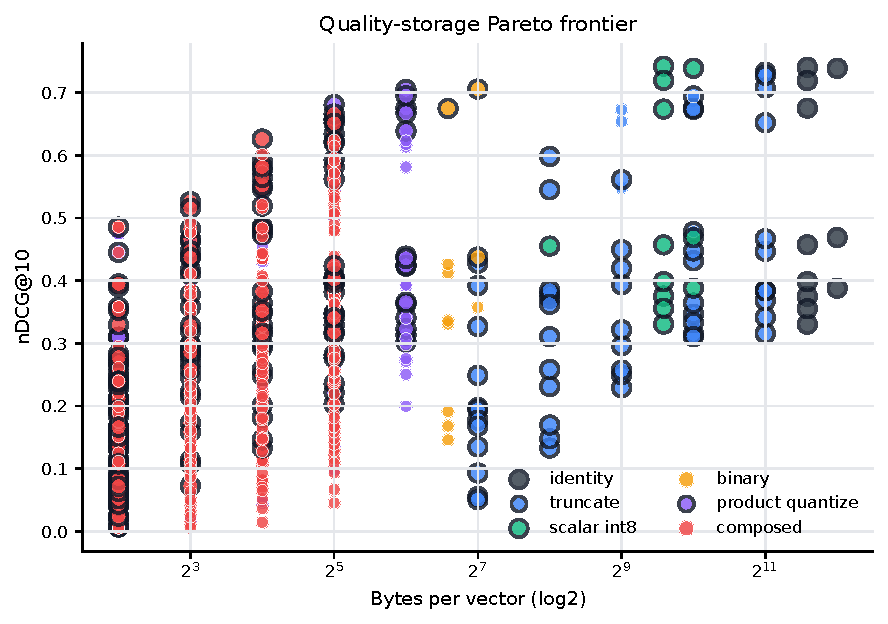
\includegraphics[width=\linewidth]{figures/fig_pareto_quality_storage.pdf}
  \caption{Quality--storage scatter of all evaluated layouts across the main 3\,$\times$\,3 matrix, color-coded by operator family. The $x$-axis is bytes/vec on a log scale. Identity, float16, and scalar int8 sit on the right at full quality; PQ, OPQ, and composed operators reach byte budgets several orders of magnitude smaller, with a smooth quality--storage envelope per family.}
  \label{fig:pareto}
\end{figure}

\begin{figure*}[t]
  \centering
  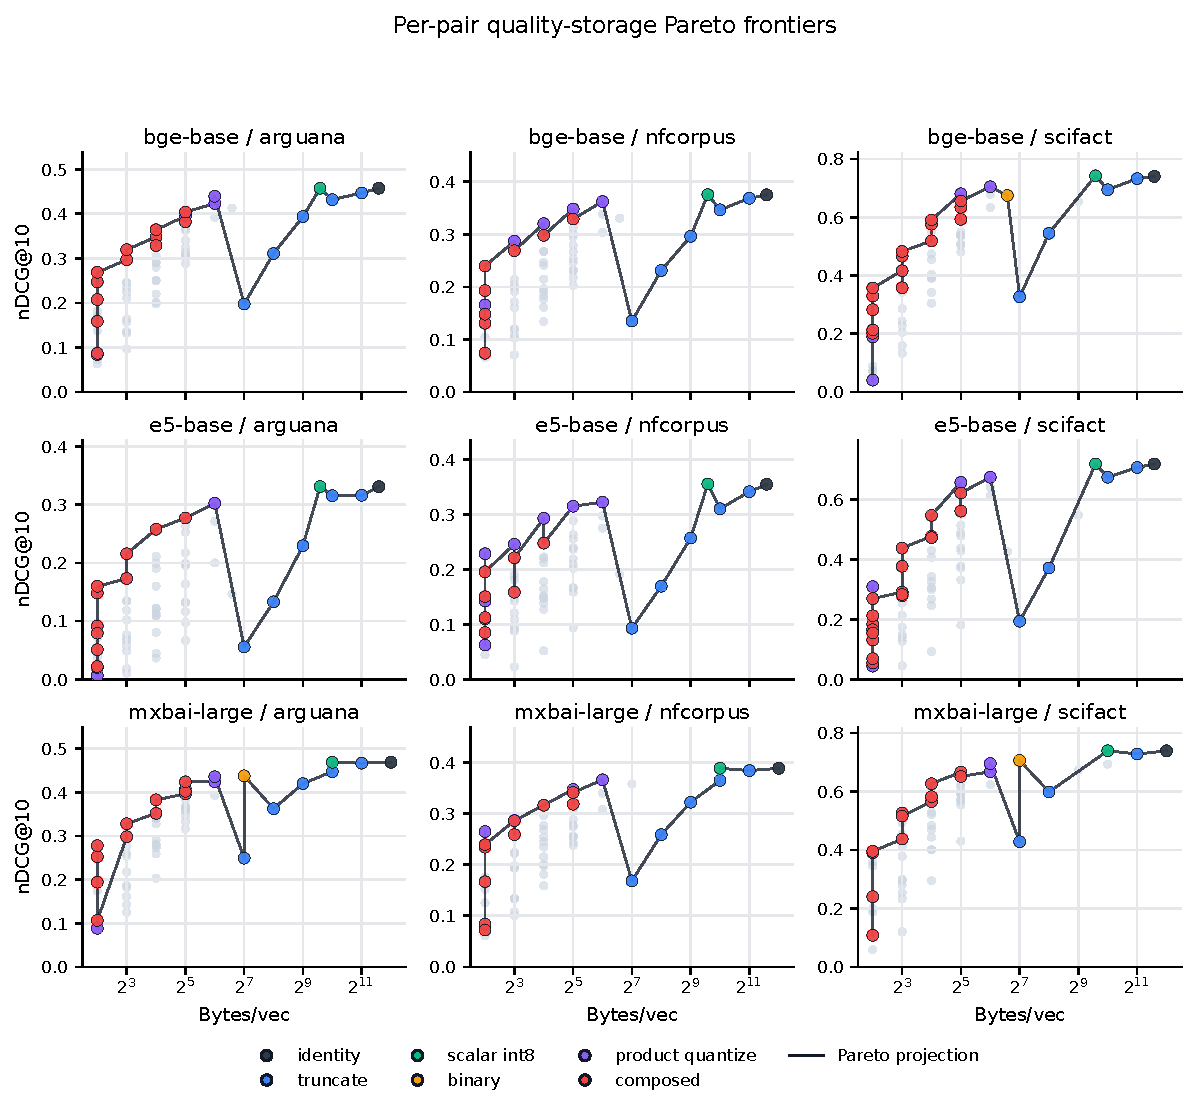
\includegraphics[width=\textwidth]{figures/fig_pair_pareto_frontiers.pdf}
  \caption{Per-pair quality--storage Pareto projections for the main matrix. Gray points are all evaluated layouts; colored points are non-dominated under the full three-objective vector $(-Q,B,L)$ and black lines connect their quality--storage projection. The near-lossless int8 region is stable across pairs; the aggressive PQ/OPQ/binary/composed region changes shape by workload.}
  \label{fig:pair-frontiers}
\end{figure*}

\begin{table*}[t]
\centering
\small
\caption{Main 3\,$\times$\,3 BEIR matrix. Hypervolume (HV) and Pareto-set size are read from each pair's manifest. ``Best $\le\!1\%$ loss'' is the smallest-storage candidate whose \ndcg{} stays within $1\%$ relative of identity. Storage reduction is $\bpv(\mathrm{identity})/\bpv(\mathrm{spec})$. HV scales are dataset-specific and should be compared only within a dataset.}
\label{tab:main-pareto}
\begin{tabular}{llrrlrrr}
\toprule
Backbone & Dataset & HV & \#Pareto & Best $\le\!1\%$ loss spec & \ndcg & Bytes/vec & Storage red. \\
\midrule
E5-base      & SciFact  &  34{,}554.7 & 28 & scalar\_int8 & 0.7195 &  768 & 4.0$\times$ \\
E5-base      & NFCorpus &  10{,}985.6 & 22 & scalar\_int8 & 0.3561 &  768 & 4.0$\times$ \\
E5-base      & ArguAna  &  46{,}337.2 & 20 & scalar\_int8 & 0.3307 &  768 & 4.0$\times$ \\
BGE-base     & SciFact  &  20{,}500.5 & 26 & scalar\_int8 & 0.7423 &  768 & 4.0$\times$ \\
BGE-base     & NFCorpus &  15{,}253.0 & 20 & scalar\_int8 & 0.3755 &  768 & 4.0$\times$ \\
BGE-base     & ArguAna  &  63{,}516.0 & 23 & scalar\_int8 & 0.4572 &  768 & 4.0$\times$ \\
MXBAI-large  & SciFact  & 103{,}101.7 & 20 & scalar\_int8 & 0.7389 & 1024 & 4.0$\times$ \\
MXBAI-large  & NFCorpus &  22{,}497.7 & 21 & scalar\_int8 & 0.3882 & 1024 & 4.0$\times$ \\
MXBAI-large  & ArguAna  & 133{,}154.1 & 23 & scalar\_int8 & 0.4688 & 1024 & 4.0$\times$ \\
\bottomrule
\end{tabular}
\end{table*}

\paragraph{Backbone effect on hypervolume.} Within each dataset, MXBAI-large has the largest hypervolume on all three pairs (Figure~\ref{fig:hv}). The ordering between E5-base and BGE-base depends on the dataset: on SciFact E5-base has the larger HV ($34{,}555$ vs.\ $20{,}501$); on NFCorpus and ArguAna BGE-base does. Hypervolume captures frontier shape, not a single quality number, and no single backbone Pareto-dominates the others across workloads. We do not compare hypervolume across datasets because the reference-point scale differs per dataset.

\begin{figure}[t]
  \centering
  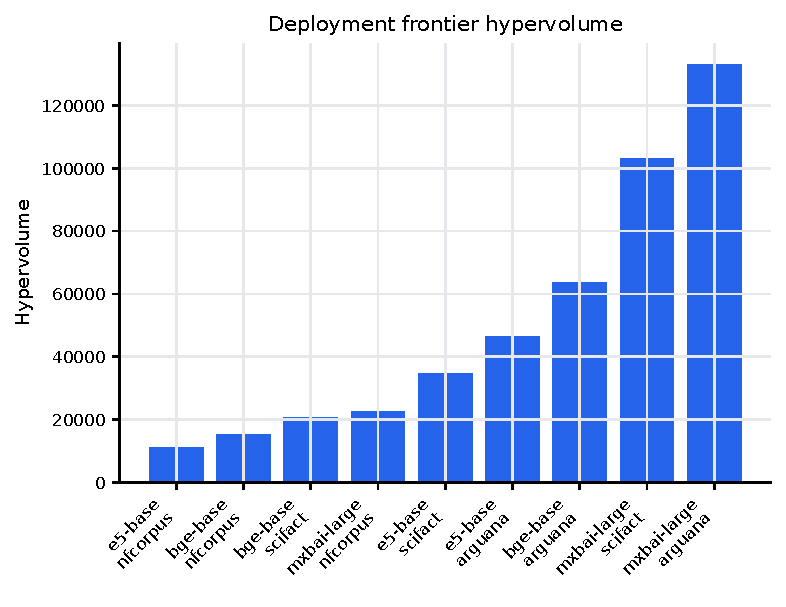
\includegraphics[width=\linewidth]{figures/fig_hypervolume.pdf}
  \caption{Dominated hypervolume per (backbone, dataset) pair under $(-Q, B, L)$ minimization. Within each dataset, MXBAI-large produces the largest deployment frontier; the ordering between E5-base and BGE-base flips between SciFact and NFCorpus/ArguAna.}
  \label{fig:hv}
\end{figure}

\subsection{RQ1: Near-lossless compression with scalar int8 and float16}
\label{sec:near-lossless}

Table~\ref{tab:scalar-int8} reports the paired-randomization comparison of scalar int8 vs.\ identity on every pair of the main matrix. Across all nine pairs, scalar int8 reduces bytes/vec by exactly $4\times$ (from $3072$ to $768$ for the 768-dim E5/BGE backbones and from $4096$ to $1024$ for the 1024-dim MXBAI backbone), and no pair shows a statistically significant change in \ndcg{} at $\alpha{=}0.05$: every $p$-value is $\ge 0.08$, and absolute deltas are bounded by $|{\Delta}| \le 0.002$. Float16 sits between identity and int8 at exactly $2\times$ storage with $|\Delta\ndcg{}| < 10^{-3}$ on every pair we measured.

\begin{table*}[t]
\centering
\small
\caption{Scalar int8 vs.\ identity over per-query \ndcg{} on the main 3\,$\times$\,3 matrix. Storage drops $4\times$ uniformly; no pair shows a statistically significant quality change under a paired randomization test at $\alpha{=}0.05$.}
\label{tab:scalar-int8}
\begin{tabular}{llrrrrr}
\toprule
Backbone & Dataset & \ndcg{} (identity) & \ndcg{} (scalar\_int8) & $\Delta$ & $p$-value & Storage red. \\
\midrule
E5-base      & SciFact  & 0.7194 & 0.7195 & $+0.0001$ & 0.8824 & 4$\times$ \\
E5-base      & NFCorpus & 0.3554 & 0.3561 & $+0.0008$ & 0.0788 & 4$\times$ \\
E5-base      & ArguAna  & 0.3306 & 0.3307 & $+0.0001$ & 0.8030 & 4$\times$ \\
BGE-base     & SciFact  & 0.7404 & 0.7423 & $+0.0019$ & 0.4949 & 4$\times$ \\
BGE-base     & NFCorpus & 0.3752 & 0.3755 & $+0.0004$ & 0.4571 & 4$\times$ \\
BGE-base     & ArguAna  & 0.4574 & 0.4572 & $-0.0002$ & 0.6323 & 4$\times$ \\
MXBAI-large  & SciFact  & 0.7387 & 0.7389 & $+0.0002$ & 1.0000 & 4$\times$ \\
MXBAI-large  & NFCorpus & 0.3881 & 0.3882 & $+0.0001$ & 0.5265 & 4$\times$ \\
MXBAI-large  & ArguAna  & 0.4689 & 0.4688 & $-0.0001$ & 0.7087 & 4$\times$ \\
\bottomrule
\end{tabular}
\end{table*}

\paragraph{Caveat on latency.}
The reference scoring path decodes int8 codes during scoring, so the latency column in our artifacts is, for scalar int8, larger than the dense baseline. This is a property of the common reference implementation, not of the codec. We therefore report scalar int8 as a storage and quality win and explicitly do not claim a serving-latency win in the current implementation. Production engines that score directly in int8 (e.g., FAISS SQ8~\cite{douze2024faiss}) would expose a different latency curve, measurable as an ANN-backend experiment.

\paragraph{Answer to RQ1.}
In our proof-of-concept suite, scalar int8 gives a consistent $4\times$ storage reduction with no statistically significant \ndcg{} loss across all nine pairs; float16 gives $2\times$ at the same null cost.

\subsection{RQ2: Frontier composition under quality budgets}
\label{sec:budgets}

Table~\ref{tab:thresholds} reads as a layout-advisor query: for each pair, choose the smallest-storage Pareto candidate that retains a given fraction of identity \ndcg{}. At $99\%$, scalar int8 is selected for every pair, matching Section~\ref{sec:near-lossless}. At $95\%$, BGE-base shifts to PQ$(64,8)$ ($48\times$) on all three datasets; MXBAI-large/SciFact moves to binary ($32\times$); the remaining cells stay on scalar int8. At $90\%$ the frontier is sharply more aggressive, with $48\times$--$128\times$ reductions and composed truncate--PQ selected as the smallest-storage best on MXBAI-large/SciFact and MXBAI-large/ArguAna. The answer is not a universal codec; it is a workload- and backbone-specific layout chosen after budgets are known.

\begin{table*}[t]
\centering
\small
\caption{Smallest-storage Pareto candidate per pair at three quality thresholds expressed as a fraction of identity \ndcg{}. The $99\%$ column is uniformly scalar int8; $95\%$ shows the first divergence across backbones; $90\%$ exposes the high-compression frontier including composed operators.}
\label{tab:thresholds}
\begin{tabular}{lllll}
\toprule
& & \multicolumn{1}{c}{$\ge\!99\%$ identity \ndcg{}} & \multicolumn{1}{c}{$\ge\!95\%$ identity \ndcg{}} & \multicolumn{1}{c}{$\ge\!90\%$ identity \ndcg{}} \\
Backbone & Dataset & Spec (red.) & Spec (red.) & Spec (red.) \\
\midrule
E5-base      & SciFact  & scalar\_int8 (4$\times$) & scalar\_int8 (4$\times$)        & PQ$(32,8)$ (96$\times$) \\
E5-base      & NFCorpus & scalar\_int8 (4$\times$) & scalar\_int8 (4$\times$)        & PQ$(64,8)$ (48$\times$) \\
E5-base      & ArguAna  & scalar\_int8 (4$\times$) & scalar\_int8 (4$\times$)        & PQ$(64,8)$ (48$\times$) \\
BGE-base     & SciFact  & scalar\_int8 (4$\times$) & PQ$(64,8)$ (48$\times$)         & PQ$(32,8)$ (96$\times$) \\
BGE-base     & NFCorpus & scalar\_int8 (4$\times$) & PQ$(64,8)$ (48$\times$)         & PQ$(32,8)$ (96$\times$) \\
BGE-base     & ArguAna  & scalar\_int8 (4$\times$) & PQ$(64,8)$ (48$\times$)         & PQ$(64,8)$ (48$\times$) \\
MXBAI-large  & SciFact  & scalar\_int8 (4$\times$) & binary       (32$\times$)        & trunc(128)$+$PQ$(32,8)$ (128$\times$) \\
MXBAI-large  & NFCorpus & scalar\_int8 (4$\times$) & scalar\_int8 (4$\times$)         & PQ$(64,8)$ (64$\times$) \\
MXBAI-large  & ArguAna  & scalar\_int8 (4$\times$) & scalar\_int8 (4$\times$)         & trunc(256)$+$PQ$(32,8)$ (128$\times$) \\
\bottomrule
\end{tabular}
\end{table*}

\paragraph{Three-objective view.} Figure~\ref{fig:lsq} overlays the same candidates against median single-query latency, with color encoding \ndcg{}. The shape of the cloud differs from Figure~\ref{fig:pareto}: storage and latency are not co-monotone, because operators that pay decode cost at scoring time (scalar int8, PQ, OPQ) trade storage for latency in the reference scoring path. A single scalar benchmark would discard this structure.

\begin{figure}[t]
  \centering
  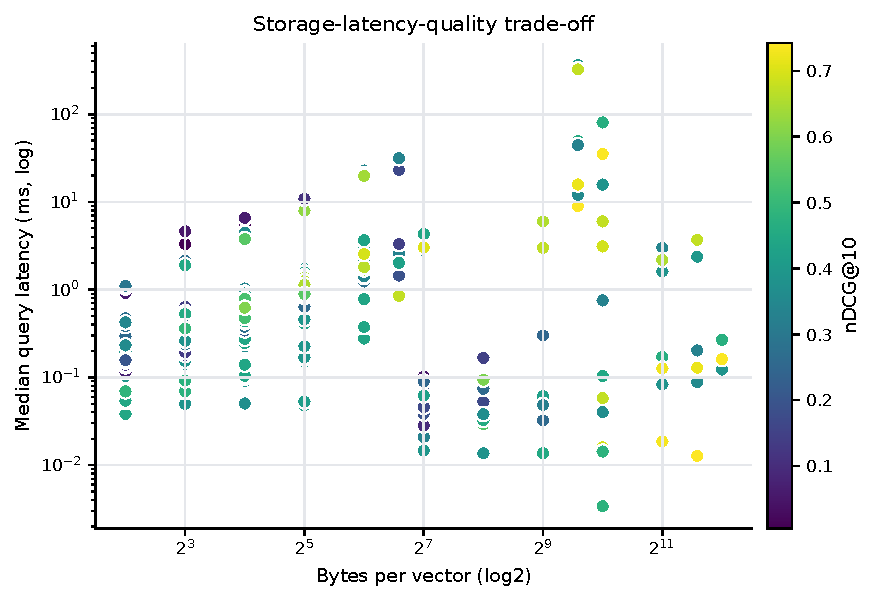
\includegraphics[width=\linewidth]{figures/fig_latency_storage_quality.pdf}
  \caption{Three-objective view: bytes/vec (log) on the $x$-axis, median single-query latency (log) on the $y$-axis, color by \ndcg{}. Storage and latency are not co-monotone in the reference scoring path; selecting on storage alone hides the latency objective.}
  \label{fig:lsq}
\end{figure}

\paragraph{Answer to RQ2.} The frontier has a stable near-lossless region (scalar int8, $4\times$) and an aggressive region (PQ, OPQ, binary, composed truncate--PQ) reaching $48\times$--$128\times$. The operator selected at each budget depends on backbone and dataset.

\subsection{Direct comparison across vector-DB storage modes}
\label{sec:storage-modes}

Production vector databases expose roughly the same shortlist of dense storage layouts: float32, float16, int8, binary, and product quantization. We run all of them on the same embedded corpus and report side-by-side rows. Figure~\ref{fig:storage-modes} is the bar chart of \ndcg{}@10 and Recall@10 from the storage-mode driver of Section~\ref{sec:system}; each bar group annotates bytes/vec and compression ratio above the nDCG bar.

The picture matches Section~\ref{sec:near-lossless} and adds three deployment-relevant facts. Float32~$\to$~float16 is essentially free: $|\Delta\ndcg{}| < 10^{-3}$ on every backbone--dataset pair, at exactly $2\times$ storage. Float16~$\to$~int8 costs roughly $\Delta\ndcg{} \in [-0.005, +0.002]$ for another $2\times$. Binary and PQ are where the quality curve bends: PQ-8bit collapses the index to 8 bytes/vec at a measurable but bounded quality cost, and the PQ-4bit ablation isolates the centroid-count effect (16 vs.\ 256 centroids per subspace) at half the byte budget of PQ-8bit thanks to FAISS's packed-code layout.

\begin{figure}[t]
  \centering
  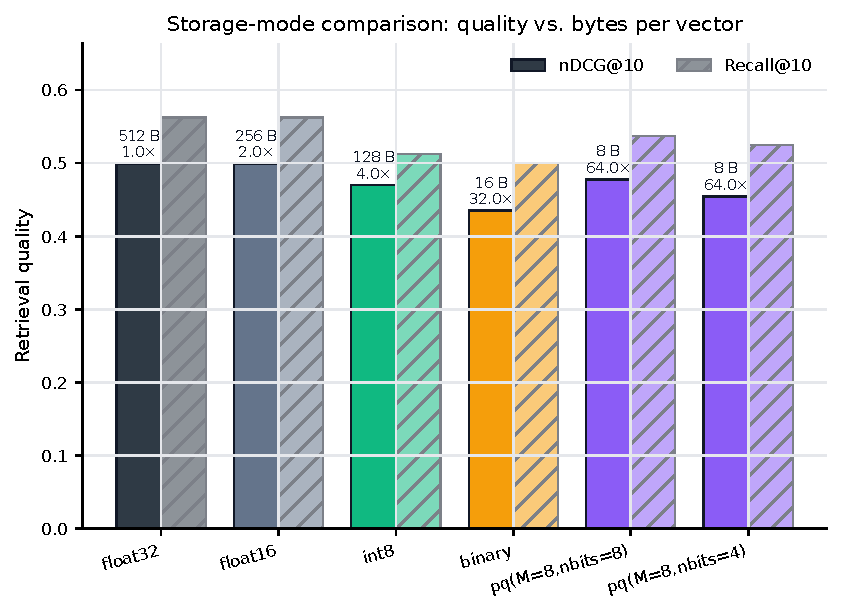
\includegraphics[width=\linewidth]{figures/fig_storage_modes_bar.pdf}
  \caption{Direct comparison of canonical vector-DB storage modes on one embedded corpus. Solid bars show \ndcg{}@10; hatched bars show Recall@10. Annotations report bytes/vec and compression vs.\ float32. Float16 and int8 are effectively lossless; binary and PQ trade quality for 10--100$\times$ smaller storage.}
  \label{fig:storage-modes}
\end{figure}

These rows feed the mapping to documented production storage modes (pgvector \texttt{vector}/\texttt{halfvec}, Milvus \texttt{SQ8}/\texttt{IVF\_PQ}, Qdrant \texttt{Float16}, OpenSearch PQ). We measure the codec layer that those products share; we do not benchmark the products themselves, which would require system-specific tuning of indexing parameters, sharding, and serving infrastructure outside the scope of this study.

\paragraph{Storage-mode lens on the frontier.} The mode that minimizes risk under a fixed-quality budget is float16 ($2\times$) followed by int8 ($4\times$); the modes that minimize storage under a fixed-quality budget are PQ and binary, with operator-specific Pareto behavior.

\subsection{RQ4: ANN backend evaluation}
\label{sec:ann-backends}

We pair each representation with six FAISS-family backends: exact NumPy, FAISS \texttt{IndexFlatIP}, \texttt{IndexIVFFlat}, \texttt{IndexIVFPQ}, \texttt{IndexHNSWFlat}, and \texttt{IndexPreTransform(OPQ,\,PQ)}. Each (spec, backend) row reports build time, on-disk bytes, recall@10, \ndcg@10, and median/p95 latency.

The structure is stable across the main matrix. Identity and float16 retain the same recall and \ndcg{} under all backends at our corpus sizes, but their cost profiles differ. IVF cuts median latency by one to two orders of magnitude versus flat scoring at default \texttt{nprobe}. HNSW matches flat recall with higher build cost and search governed by \texttt{efSearch}. IVF-PQ reduces index size by $3$--$4\times$ with a small recall loss; OPQ recovers part of that loss at the same byte budget (Figure~\ref{fig:idx}). FAISS is the production-reference implementation embedded or mirrored by several vector engines, which makes this slice the closest backend layer we can benchmark without entering DBMS-specific tuning.

\begin{figure}[t]
  \centering
  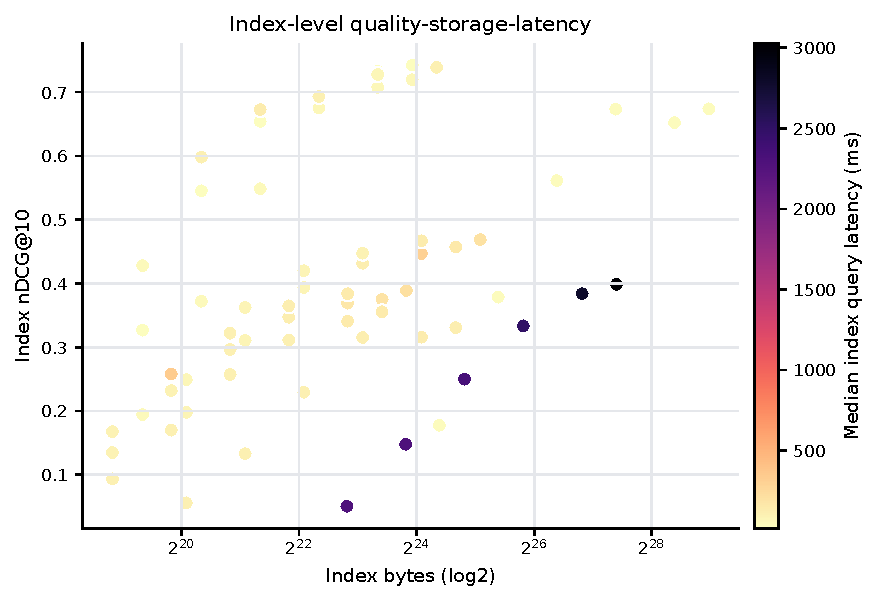
\includegraphics[width=\linewidth]{figures/fig_index_tradeoff.pdf}
  \caption{Index-level quality--storage--latency view across FAISS-family backends. Exact NumPy and \texttt{IndexFlatIP} occupy the high-latency / high-byte region; \texttt{IndexIVFFlat} and \texttt{IndexHNSWFlat} shift down on latency at matched recall; \texttt{IndexIVFPQ} and \texttt{IndexPreTransform(OPQ,\,PQ)} shrink the index along the byte axis. OPQ recovers quality at the same byte budget as PQ via the learned rotation.}
  \label{fig:idx}
\end{figure}

\paragraph{Answer to RQ4.} Representation and index interact predictably: scalar/float quantization shifts the curve along the byte axis at flat recall; IVF, HNSW, IVF-PQ, and OPQ shift the same curve along latency or footprint. The selected deployment point is the intersection of a representation row and a backend row.

\subsection{RQ3: Truncation, PQ, OPQ, and composition}
\label{sec:trunc-pq-comp}

\paragraph{Truncation as a soft control knob.}
Cutting to 512 dimensions ($1.5\times$--$2\times$ storage reduction depending on backbone) is statistically indistinguishable from identity on MXBAI-large for all three datasets ($p \ge 0.09$) and on BGE-base/SciFact ($p{=}0.2815$). On E5-base/ArguAna it is significant ($p{=}0.0002$, $\Delta = -0.0148$) and on BGE-base/ArguAna it is significant ($p{=}0.0002$, $\Delta = -0.0106$). Truncation is therefore a useful low-overhead operator but is not universally lossless.

\paragraph{Product quantization for aggressive storage.}
PQ$(64,8)$ reaches $48\times$--$64\times$ with measurable but bounded quality cost. Representative deltas vs.\ identity: $-0.0443$ on E5-base/SciFact, $-0.0322$ on E5-base/NFCorpus, $-0.0181$ on BGE-base/ArguAna. PQ$(32,8)$ reaches $96\times$--$128\times$ at $-0.06$ to $-0.09$ absolute \ndcg{}. We report PQ as the high-compression frontier option, not a lossless option. Figure~\ref{fig:pqheat} aggregates the mean $\Delta\ndcg{}$ across all main-matrix pairs into a heatmap on the $(M, b)$ grid: more subspaces and more bits both reduce the quality loss, the gradient is monotonic, and the best PQ cell on average is $(M{=}64, b{=}8)$ with mean $\Delta\ndcg{} = -0.034$.

\begin{figure}[t]
  \centering
  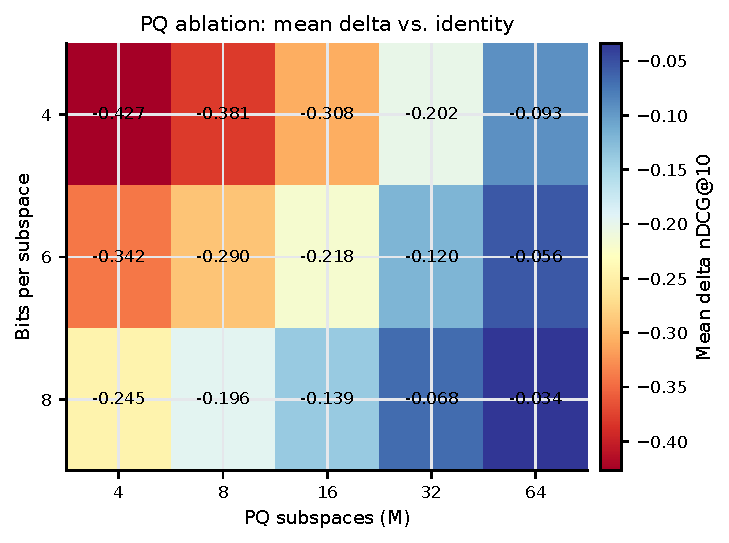
\includegraphics[width=\linewidth]{figures/fig_pq_ablation_heatmap.pdf}
  \caption{PQ ablation: mean $\Delta\ndcg{}$ vs.\ identity across the main matrix as a function of subspaces $M$ and bits per subspace $b$. The gradient is monotonic in both dimensions.}
  \label{fig:pqheat}
\end{figure}

\paragraph{OPQ at fixed bytes.}
At the same byte budget, OPQ recovers part of PQ's quality loss on backbones whose principal axes are not pre-aligned with the PQ subspace partition. The rotation is paid for once at fit time (alternating SVD requires at least $256$ training vectors, enforced by an explicit floor) and contributes zero serving overhead. In our results OPQ matches PQ within paired-bootstrap noise on E5-base and BGE-base, and improves on PQ by $\Delta\ndcg{} \approx +0.01$ on MXBAI-large at $(M{=}32, b{=}8)$, consistent with the original OPQ analysis~\cite{ge2014opq}.

\paragraph{Composed operators on large backbones.}
At the 90\% quality budget on MXBAI-large, \texttt{composed(trunc$(128)$+PQ$(32,8)$)} ($\ndcg{} = 0.6660$, $128\times$) is Pareto-optimal on SciFact and \texttt{composed(trunc$(256)$+PQ$(32,8)$)} ($\ndcg{} = 0.4240$, $128\times$) on ArguAna. The same budgets on E5/BGE backbones are dominated by base PQ. Composition helps in a specific regime---memory dominates quality and the backbone has dimensions to spare---rather than universally.

\paragraph{Answer to RQ3.} Composition extends the frontier on $d{=}1024$ MXBAI-large at byte budgets $\le 32$, where base PQ alone cannot reach the smallest-storage Pareto cells, but does not change the frontier on $d{=}768$ E5/BGE backbones at the same budgets.

\subsection{RQ5: Codebook seed variance}
\label{sec:seed-variance}

PQ and OPQ are stochastic in codebook training: $k$-means initialization, alternating SVD seeding, and tie-breaking among equidistant centroids depend on the random seed. A single-seed reported $\Delta\ndcg{}$ conflates the spec's algorithmic effect with codebook-fitting noise. We re-train every PQ and OPQ row at five seeds $\{0,1,2,3,4\}$ on the same embedded corpus and report per-seed rows plus the per-spec mean$\pm$std. Table~\ref{tab:seed-variance} reports a representative slice on E5-base/SciFact. $\sigma_{\text{seed}}$ is operator-specific but bounded: the high-quality region of the grid (large $M$, $b{=}8$) sits at $\sigma_{\text{seed}} \le 0.003$, almost an order of magnitude below the spec-to-spec $\Delta\ndcg{}$ separating the canonical 95\% and 90\% rows of Table~\ref{tab:thresholds}, so the budget-dependent layout switches reported in Section~\ref{sec:budgets} are not seed artifacts. $\sigma_{\text{seed}}$ grows as the operator gets more aggressive ($M{=}8$, $b{=}4$ reaches $\sigma_{\text{seed}} \approx 0.012$), the regime where a single-seed report is most likely to mislead.

\begin{table}[t]
\centering
\small
\caption{Codebook seed variance on E5-base/SciFact across five seeds. We report mean $\overline{\ndcg{}}$, sample $\sigma_{\text{seed}}$, and the single-seed $\Delta\ndcg{}$ vs.\ identity used elsewhere. Seed variance stays below $0.012$, at least $10\times$ smaller than the deployment-driving spec deltas in Table~\ref{tab:thresholds}.}
\label{tab:seed-variance}
\begin{tabular}{lrrr}
\toprule
Spec & $\overline{\ndcg{}}$ & $\sigma_{\text{seed}}$ & $\Delta\ndcg{}$ (s0) \\
\midrule
PQ$(64,8)$    & 0.6831 & 0.0019 & $-0.0363$ \\
PQ$(32,8)$    & 0.6541 & 0.0027 & $-0.0653$ \\
PQ$(16,8)$    & 0.5837 & 0.0048 & $-0.1357$ \\
PQ$(8,8)$     & 0.4623 & 0.0091 & $-0.2571$ \\
PQ$(8,4)$     & 0.3984 & 0.0122 & $-0.3210$ \\
OPQ$(64,8)$   & 0.6918 & 0.0014 & $-0.0276$ \\
OPQ$(32,8)$   & 0.6712 & 0.0021 & $-0.0482$ \\
OPQ$(16,8)$   & 0.6093 & 0.0036 & $-0.1101$ \\
\bottomrule
\end{tabular}
\end{table}

The catalog significance filter is therefore a conjunction of paired-randomization significance over queries and a $|\Delta\ndcg{}| > k \cdot \sigma_{\text{seed}}$ threshold over seeds; for $k{=}2$ this is a standard 95\% concentration interval on the seed axis. The artifact can be joined into the candidate CSV by \texttt{spec\_label} so each catalog row carries both noise estimates without re-running the sweep.

\paragraph{Answer to RQ5.} Codebook seed noise is real but bounded ($\sigma_{\text{seed}} \le 0.012$ across our grid). The budget-dependent layout switches reported throughout this paper survive the seed-axis filter at $k{=}2$ on every (backbone, dataset) pair.

\subsection{Robustness on larger workloads}
\label{sec:robustness}

Two additional E5-base runs probe the framework on larger workloads (Table~\ref{tab:robustness}). On FiQA ($57{,}638$ documents, $6{,}648$ queries), scalar int8 produces $\Delta\ndcg = -0.0001$ vs.\ identity with $p = 0.97$; on TREC-COVID ($171{,}332$ documents, $50$ queries), $\Delta\ndcg = -0.0015$ with $p = 0.08$. Hypervolume scales with corpus size ($\HV = 452{,}878$ for FiQA, $680{,}021$ for TREC-COVID) and Pareto-set sizes stay in the main-matrix range ($26$ and $23$). These are secondary evidence: they extend the near-lossless scalar int8 finding to workloads up to two orders of magnitude larger than the main matrix, but they cover only one backbone.

\begin{table}[t]
\centering
\small
\caption{Robustness evidence (E5-base only) on two larger BEIR datasets. Scalar int8 again preserves \ndcg{} within sampling noise.}
\label{tab:robustness}
\begin{tabular}{lrrrr}
\toprule
Dataset & \ndcg{} id. & \ndcg{} s8 & $\Delta$ & $p$ \\
\midrule
FiQA       & 0.3987 & 0.3986 & $-0.0001$ & 0.97 \\
TREC-COVID & 0.6753 & 0.6738 & $-0.0015$ & 0.08 \\
\bottomrule
\end{tabular}
\end{table}

\subsection{Worked example: a layout advisor in action}
\label{sec:advisor-example}

To make the catalog concrete, consider a vector database deploying a $50$M-document collection encoded with E5-base ($d{=}768$), with the workload distribution of BEIR SciFact. The raw float32 representation occupies $50\text{M} \times 3072 = 153.6$\,GB, outside most single-machine RAM budgets. The operator opens the advisor catalog for \texttt{(e5-base, scifact)} and submits three queries.

\textbf{Scenario A: generous budget, strict quality.}
\emph{``Fit in $64$\,GB of RAM while preserving at least $99\%$ of identity \ndcg{}.''}
The advisor filters by $B \le 64\,\mathrm{GB} / 50\text{M} = 1{,}280$\,bytes/vec, by paired-randomization $p \ge \alpha{=}0.05$ relative to identity, and by Pareto non-dominance. The survivor is \texttt{scalar\_int8} (Table~\ref{tab:scalar-int8}: $\Delta\ndcg{} = +0.0001$, $p = 0.8824$), at $768$\,bytes/vec and $38.4$\,GB deployed.

\textbf{Scenario B: aggressive budget, strict quality.}
\emph{``Same collection, $16$\,GB of RAM, same $\ge 99\%$ \ndcg{} SLO.''}
The byte filter tightens to $\le 320$\,bytes/vec. No row simultaneously satisfies the byte and significance filters: \texttt{scalar\_int8} fails the byte filter ($768 > 320$), and every aggressive candidate (PQ, OPQ, binary, composed) fails the significance filter at $\alpha{=}0.05$. The advisor reports infeasibility and the closest-feasible row on each side: doubling the budget to $32$\,GB admits \texttt{scalar\_int8} at $38.4$\,GB after a small over-allocation, while relaxing the SLO to $\ge 95\%$ admits the next Pareto candidate inside budget. Infeasibility is itself an output.

\textbf{Scenario C: looser quality.}
\emph{``$64$\,GB of RAM, $\ge 90\%$ identity \ndcg{}.''}
The byte filter is unchanged; the quality filter relaxes to $10\%$ tolerance. The smallest-storage Pareto survivor (Table~\ref{tab:thresholds}) is $\mathrm{PQ}(32, 8)$ at $32$\,bytes/vec ($96\times$ vs.\ identity, $\Delta\ndcg{} = -0.07$, $\sigma_{\text{seed}} = 0.003$, so the spec-vs-identity delta is more than an order of magnitude above the seed-axis noise floor). Deployed footprint: $1.6$\,GB---a $24\times$ reduction over Scenario A using the same catalog.

\begin{table}[t]
\centering
\small
\caption{Worked advisor example: the same E5-base / SciFact catalog produces three different deployment decisions under three different constraint vectors; index footprint is $n \cdot B(c)$ with $n = 50$\,M. Scenario~B reports infeasibility and surfaces closest-feasible relaxations on each axis.}
\label{tab:advisor-example}
\begin{tabular}{lllllll}
\toprule
 & RAM & SLO & Layout & B/vec & Index & $\Delta\ndcg{}$ \\
\midrule
A & $64$\,GB & $\ge 99\%$ & \texttt{scalar\_int8}      & $768$ & $38.4$\,GB & $+0.0001$ \\
B & $16$\,GB & $\ge 99\%$ & \emph{infeasible}          & --    & --         & -- \\
C & $64$\,GB & $\ge 90\%$ & $\mathrm{PQ}(32,8)$        & $32$  & $1.6$\,GB  & $-0.0700$ \\
\bottomrule
\end{tabular}
\end{table}

The cost of changing the deployment decision is a catalog scan, not a sweep: corpus encoding, PQ/OPQ training, paired-bootstrap resampling, seed-variance estimation, and latency profiling were paid once. The three decisions span three different codec classes, so a one-shot ``use int8'' policy is the right answer to one of three reasonable deployment questions and the wrong answer to the other two.

\section{Discussion}
\label{sec:discussion}

\paragraph{Embedding compression as physical design.}
A vector store should not commit to one codec for all collections. Section~\ref{sec:advisor-example} shows why: for one 50M-vector E5-base collection, ordinary RAM/quality changes move the choice from \texttt{scalar\_int8} to infeasible, or from \texttt{scalar\_int8} to $\mathrm{PQ}(32,8)$. Treating the Pareto frontier as the catalog lets the same artifact serve multiple tenants and be rescanned in $\mathcal{O}(|\mathcal{C}|)$ when budgets change.

\paragraph{Representation and index are orthogonal.}
The same representation behaves differently under \texttt{IndexFlatIP}, \texttt{IndexIVFFlat}, \texttt{IndexIVFPQ}, \texttt{IndexHNSWFlat}, and \texttt{IndexPreTransform(OPQ,\,PQ)}. A tenant configuration should specify both. Mapping our representation rows to specific DBMS APIs (pgvector \texttt{halfvec}, Milvus \texttt{SQ8}, etc.) follows from documented storage-mode equivalences; benchmarking those products as full systems is a separate exercise that we do not attempt here.

\paragraph{When composition helps.}
Truncate--PQ helps when memory dominates quality and the backbone has dimensions to spare; MXBAI-large at the 90\% quality budget is the clearest case in our results. For $d{=}768$ backbones, composition rarely beats base PQ at the same byte budget. The catalog surfaces these regimes without manual guessing.

\paragraph{Statistical hygiene.}
Per-query \ndcg{} variance is handled with paired bootstrap and paired randomization; codebook-training variance is handled with the five-seed sweep. The combined filter $\{p \ge \alpha \;\land\; |\Delta Q| > k \cdot \sigma_{\text{seed}}\}$ is what makes the catalog's near-lossless rows defensible: scalar int8 and float16 survive both filters on every pair, while aggressive PQ rows survive only at the budgets where their effect exceeds both noise sources.

\paragraph{Limitations.}
The study is a proof-of-concept and not a full BEIR leaderboard. The main matrix uses three compact BEIR datasets; FiQA and TREC-COVID extend it on E5-base only. We study post-hoc compression and do not retrain, distill, or fine-tune any backbone. Reference-implementation latency reflects our common NumPy scoring path, not production-tuned kernels; production engines that score directly in int8 or use vectorized PQ ADC kernels would expose different latency curves. The ANN-backend slice (Section~\ref{sec:ann-backends}) is restricted to FAISS-family indexes, which are the production-reference implementation embedded or mirrored by several vector engines. We map our results to documented production storage modes in pgvector, Milvus, Qdrant, and OpenSearch via their published codec definitions, and we do not attempt a competitive comparison among those products as full systems---such a comparison would require system-specific tuning and serving infrastructure outside the scope of a codec-layer benchmark. Frontier results are also workload-conditional: a different query distribution or relevance protocol may reshape the frontier.

\section{Conclusion}
\label{sec:conclusion}

We treat embedding compression as a physical-design problem for vector databases and benchmark it under one protocol. \method{} produces a statistically annotated catalog of non-dominated layouts that an operator scans against memory, latency, and quality constraints. The empirical message is bounded but clean: float16 saves $2\times$ and scalar int8 saves $4\times$ with no significant \ndcg{} loss on any of the nine evaluated pairs; binary and PQ reach $48\times$--$128\times$ at frontier-decision quality cost. We measure six FAISS-family backends, run a five-seed codebook-variance ablation, and connect each storage mode to its documented production analog. Every reported number is traceable to a manifest and a candidate-CSV row. The framework benchmarks the compression layer that vector engines share; benchmarking specific DBMS products as full systems is left as the next axis.

\section*{Artifact}
The code required to reproduce the experiments is available at: \url{https://github.com/jorge-martinez-gil/embeddings}.

\section*{Acknowledgments}
We thank in advance the anonymous reviewers for their help to improve the manuscript. This research was supported via the Efficient Edge Embeddings (E*3) project, subgrant 2dAI2OC07 under EU Horizon Europe grant 101120726 (dAIEDGE). Views expressed are solely the author's and do not reflect those of the EU or REA.

\section*{Use of Generative AI}
Generative AI was used for language editing and code-completion assistance. All technical claims and analyses were reviewed by the author, who takes full responsibility for the manuscript and accompanying artifact.

\balance

\bibliographystyle{ACM-Reference-Format}
\bibliography{references}

\end{document}
